% Conference slides for the DSMC+PINN_AUX-BO convergence study (Beamer)
\documentclass[aspectratio=169]{beamer}
\usetheme{Madrid}
\usecolortheme{default}
\usepackage{graphicx}
\usepackage{amsmath}
\graphicspath{{figures/}}

\title[Convergence of DSMC--PINN--BO Pipeline]{Convergence of a Multifidelity DSMC--PINN--Bayesian Pipeline for HIAD Analysis}
\author{Wahyu Suryo Samudro}
\institute{Institut Teknologi Bandung\\Correspondence: albertstarfield@protonmail.com}
\date{2026}


\setbeamertemplate{footline}{
  \leavevmode\hbox{%
  \begin{beamercolorbox}[wd=.333333\paperwidth,ht=2.25ex,dp=1ex,center]{author in head/foot}%
    \usebeamerfont{author in head/foot}\insertshortauthor%
  \end{beamercolorbox}%
  \begin{beamercolorbox}[wd=.333333\paperwidth,ht=2.25ex,dp=1ex,center]{title in head/foot}%
    \usebeamerfont{title in head/foot}\insertshorttitle%
  \end{beamercolorbox}%
  \begin{beamercolorbox}[wd=.333333\paperwidth,ht=2.25ex,dp=1ex,right]{date in head/foot}%
    \usebeamerfont{date in head/foot}Cit.: Bird 1994; Raissi 2019; Rasmussen 2006; Jones 1998\hspace*{2ex}%
  \end{beamercolorbox}}%
  \vskip0pt%
}

\begin{document}

\frame{\titlepage}

\begin{frame}{Motivation}
\begin{itemize}
\item Hypersonic inflatable aerodynamic decelerators (HIADs) need rarefied + continuum aerothermal data.
\item The StellarOrion pipeline couples DSMC, PINN, Bayesian optimization and TPS.
\item Convergence must be demonstrated at every fidelity.
\end{itemize}
\end{frame}

\begin{frame}{Pipeline overview}
\begin{itemize}
\item CadQuery geometry $\to$ SPARTA DSMC (rarefied) $\to$ PINN (continuum) $\to$ BO (geometry) $\to$ TPS (survivability).
\item Four threads: DSMC, PINN, optimization, TPS.
\item This deck shows convergence evidence for each.
\end{itemize}
\end{frame}

\begin{frame}{DSMC convergence}
\begin{itemize}
\item $2200$ particle-per-cell targets, Cartesian grid with collision pairing.
\item Cell-scale Knudsen field spans nearly three decades in the continuum band.
\item Slip band $0.01<\mathrm{Kn}<0.1$ only in the millimetre bow shock.
\item Peak stagnation heat flux $q_{\rm sg}=16.14~\mathrm{W/cm^2}$ (vs IRVE-3 $14.36$).
\end{itemize}
\end{frame}

\begin{frame}{PINN convergence}
\centering
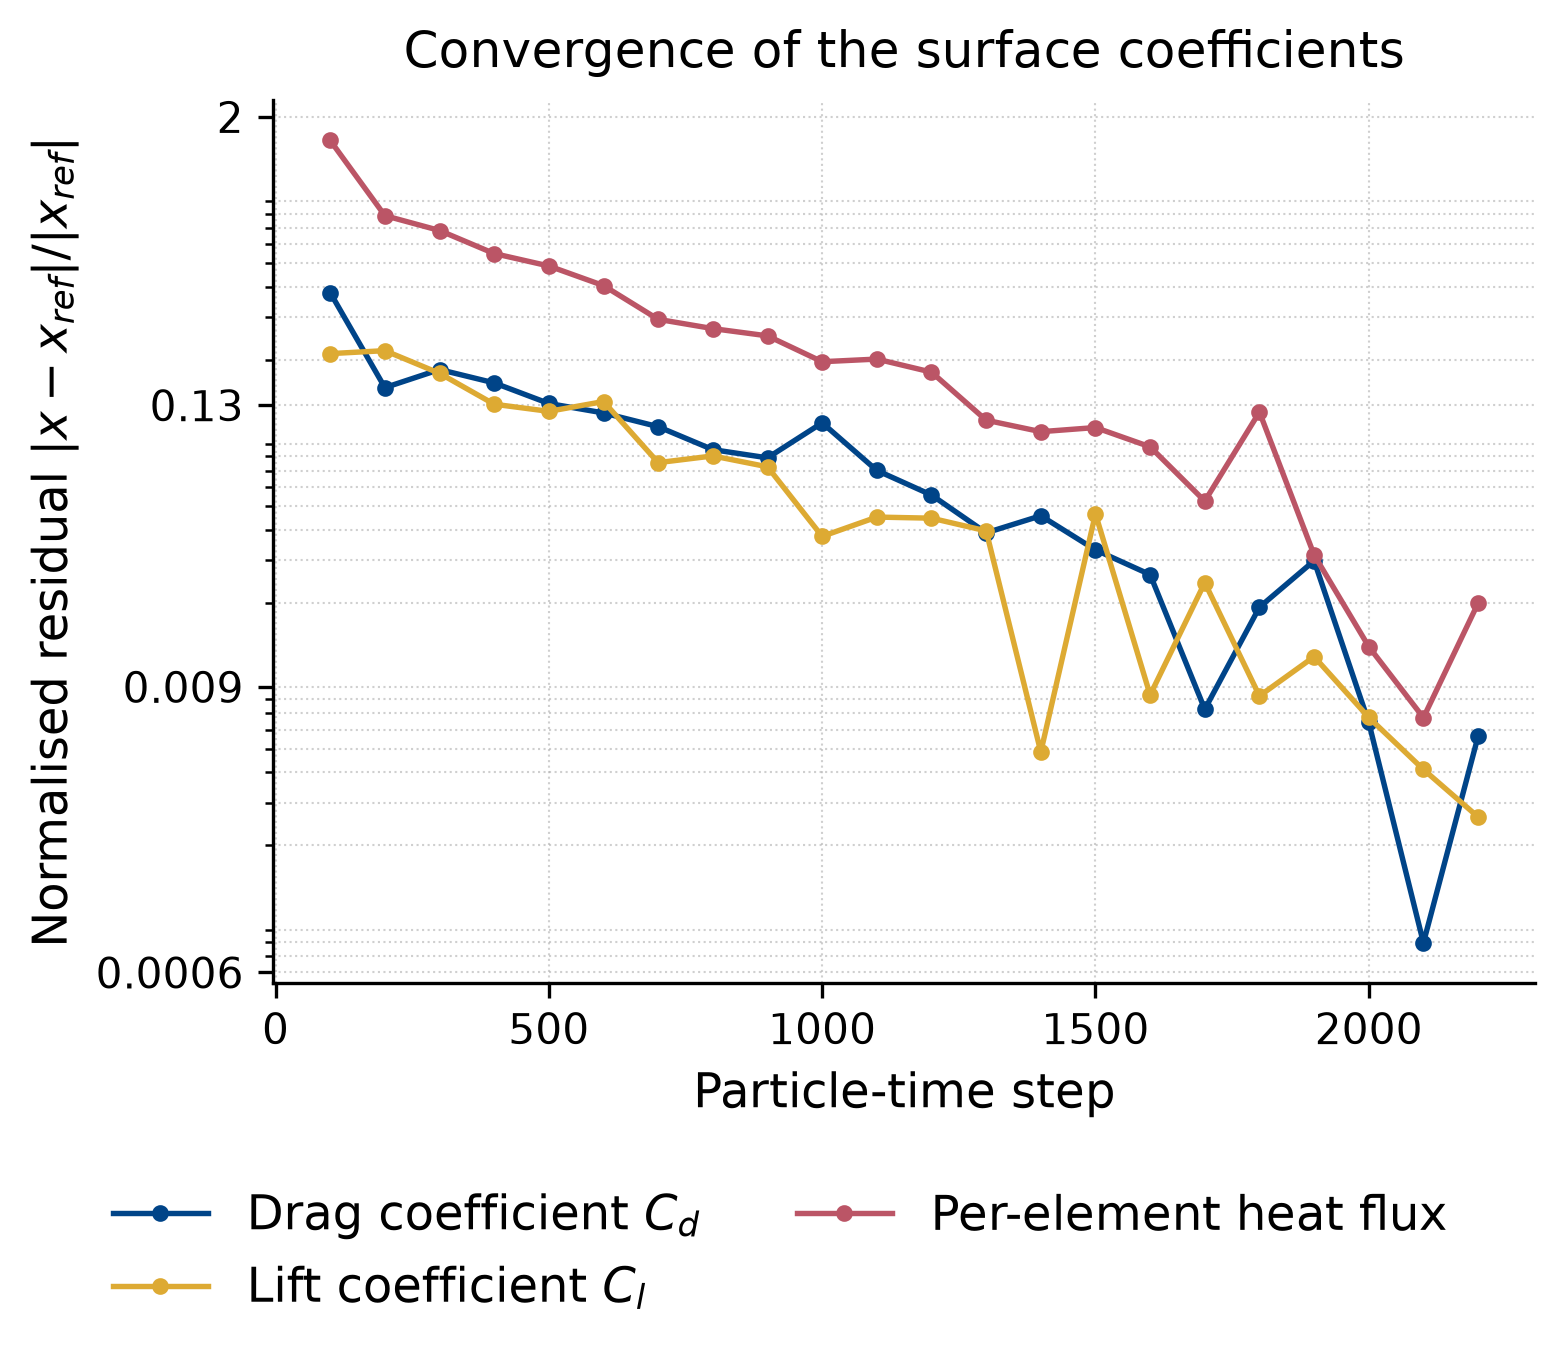
\includegraphics[width=0.5\textwidth,height=0.4\textheight,keepaspectratio]{fignew_convergence_residuals.png}
\begin{itemize}
\item Two-stage training: physics residual first, then data anchoring.
\item Kriging denoising preserves the peak stagnation quantity.
\end{itemize}
\end{frame}

\begin{frame}{Optimizer convergence}
\centering
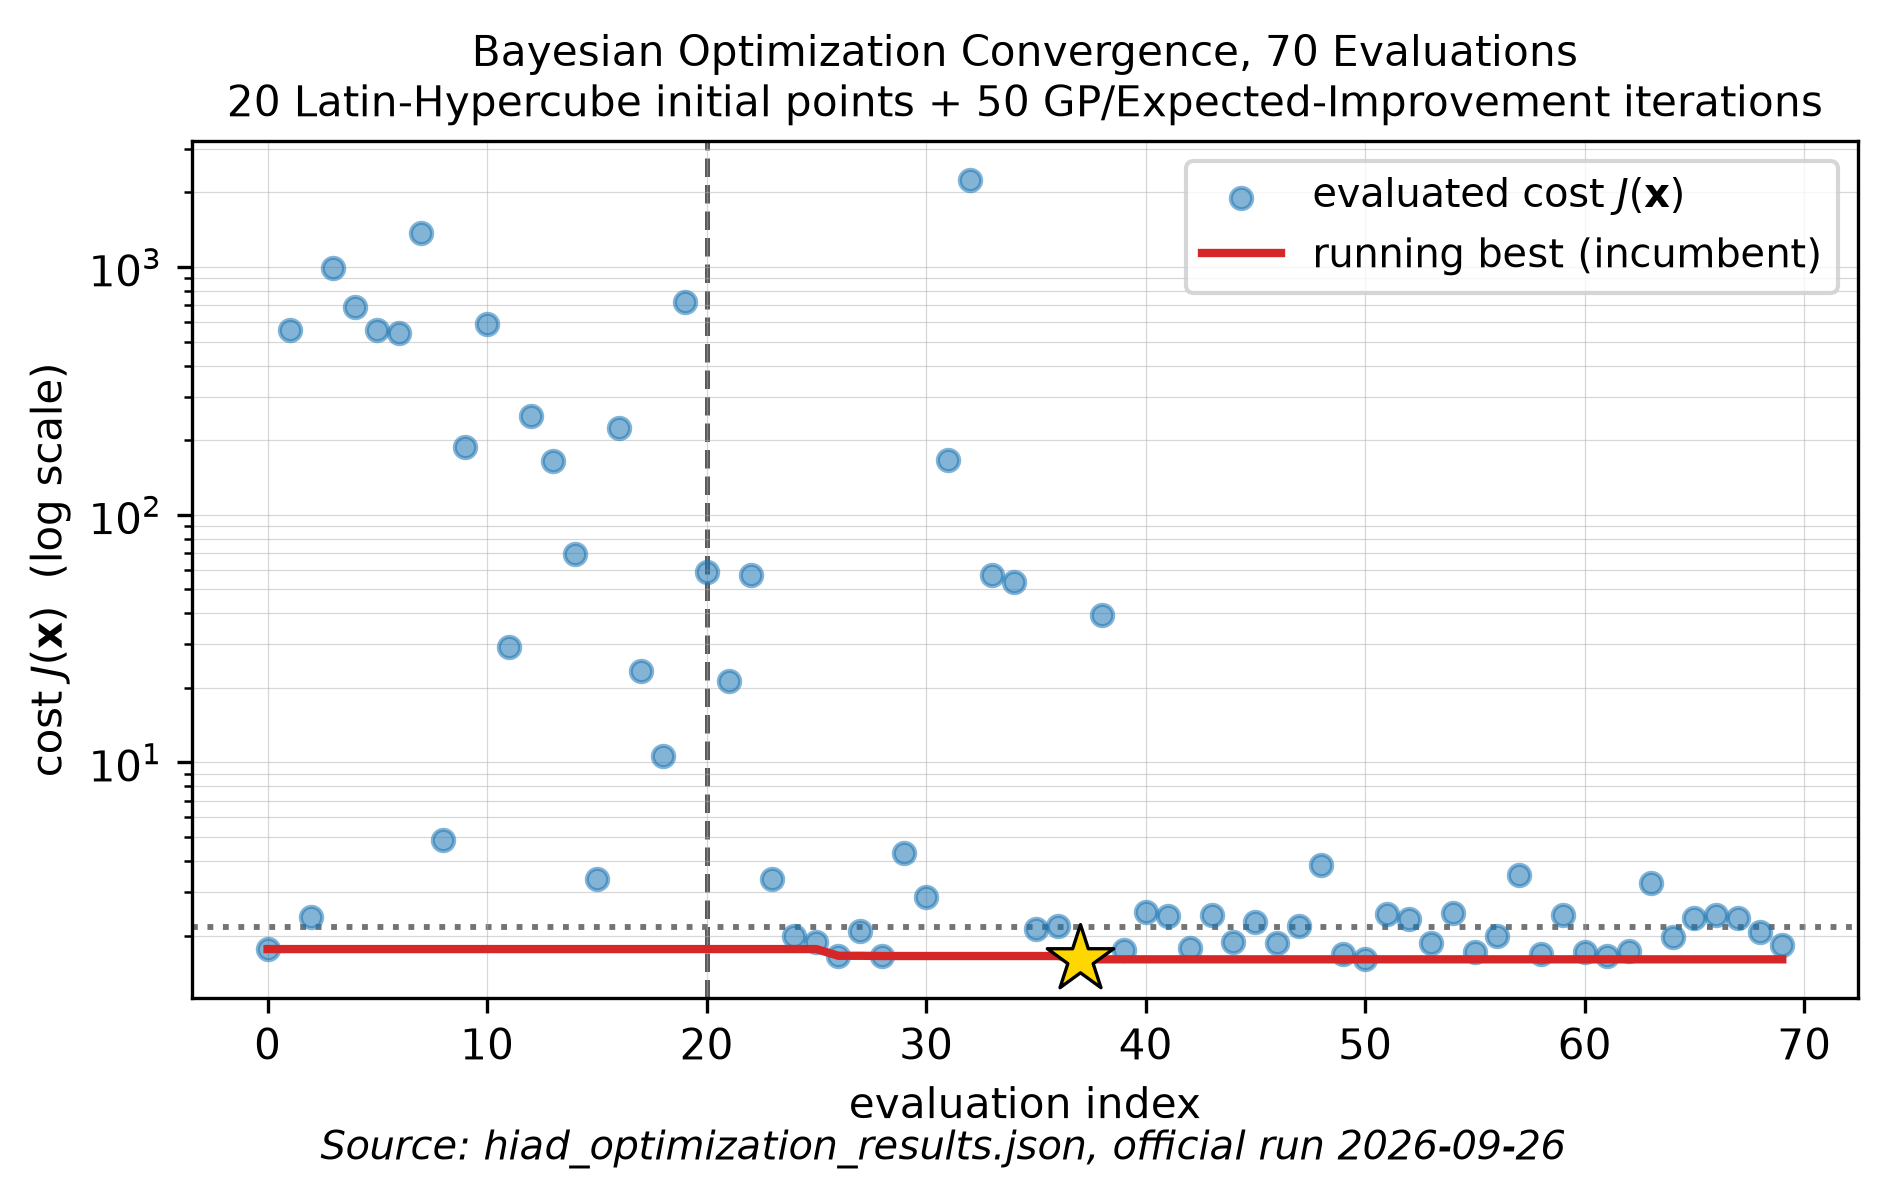
\includegraphics[width=0.5\textwidth,height=0.4\textheight,keepaspectratio]{bo_convergence.png}
\begin{itemize}
\item GP Matérn $5/2$, Expected Improvement, $10^{-9}$ denominator floor.
\item Converges in 70 evaluations to $R_N=2.9714$ m, $r_{\rm tor}=0.0885$ m, $\theta_c=40.15^\circ$.
\end{itemize}
\end{frame}

\begin{frame}{TS/TPS convergence}
\centering
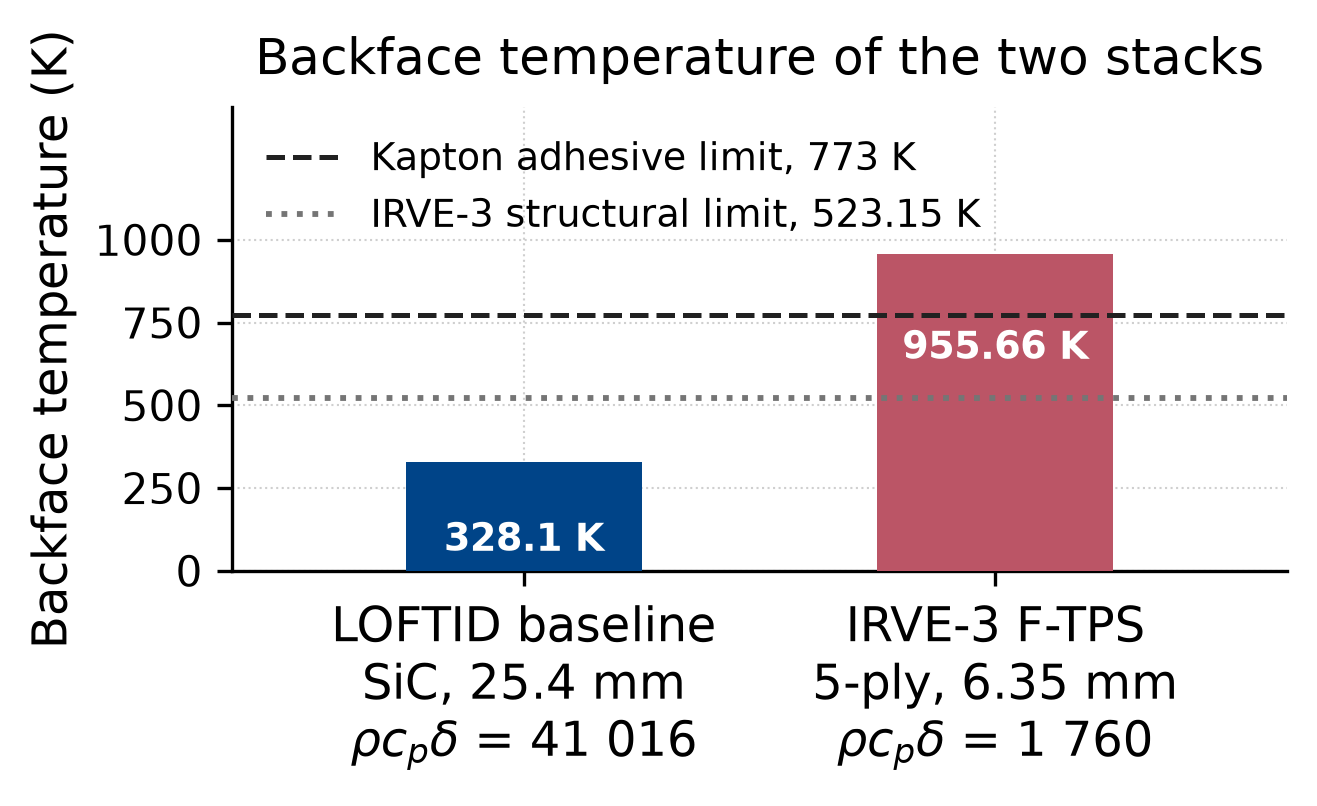
\includegraphics[width=0.5\textwidth,height=0.4\textheight,keepaspectratio]{results_tps_backface.png}
\begin{itemize}
\item Five-ply Gen-2 stack, total $7.131$ mm, settles to $T_{\rm bf}=955.66$ K.
\item Thermal pulse $Q=165.72~\mathrm{J/cm^2}$; thermal soak dominates.
\end{itemize}
\end{frame}

\begin{frame}{Conclusions}
\begin{itemize}
\item Every fidelity level converges under the reported settings.
\item Reported fluxes, optima and temperatures are trustworthy.
\item Settings become the baseline for Papers I--IV.
\end{itemize}
\end{frame}

\begin{frame}{Thank you}
\centering
Questions?\\[1em]
Wahyu Suryo Samudro\\
Institut Teknologi Bandung
\end{frame}

\end{document}
